\documentclass[aspectratio=169,9pt]{beamer}
\usetheme[progressbar=frametitle,numbering=fraction]{metropolis}
\usepackage[utf8]{inputenc}
\usepackage[T1]{fontenc}
\usepackage{amsmath,amssymb}
\usepackage{graphicx}
\usepackage{booktabs}
\usepackage{tabularx}
\usepackage{siunitx}
\usepackage{xcolor}
\sisetup{detect-all}
\definecolor{cRed}{HTML}{D62839}
\definecolor{cBlue}{HTML}{2A6FBB}
\definecolor{cGreen}{HTML}{2A9D55}
\definecolor{cOrange}{HTML}{E07B39}
\newcommand{\um}{\,\si{\micro\metre}}

\title{Model variants of the Ting fit: $E$, $\alpha$, contrast and the $E$--$\alpha$ relationship}
\subtitle{Contact point, toe force, reference time: what changes, what is robust, and what to report}
\date{Full map data\_213626 (2775 curves, $R=\SI{2.5}{\micro\metre}$) $\cdot$ synthetic curves with known $E$ and $\alpha$}
\author{}

\begin{document}
\maketitle

\begin{frame}{Summary}
\footnotesize
\begin{enumerate}
\item \textbf{The fit converges, and $E$ and $\alpha$ are separable.} Synthetic curves are recovered exactly, from the full curve and from the approach alone.
\item \textbf{The force before contact (the ``toe'') biases the results.} It is velocity dependent, likely squeeze-film drag:
 \begin{itemize}
 \item it raises the fitted $\alpha$ by +0.03 to +0.08;
 \item the bias is \emph{larger for softer curves}, which alone produces a negative $E$--$\alpha$ correlation.
 \end{itemize}
\item \textbf{$E(\SI{1}{\milli\second})$ is robust.} The fitted contact point (main) and the squeeze-film variant agree within 8\,\%, and their spatial patterns agree almost perfectly (rank correlation 0.996).\\
 The lab contact point halves $E$, and so does the elastic fit, which is not a modulus at a defined time.
\item \textbf{$E_1$ at \SI{1}{\second} is not robust.} It extrapolates the measurement over $\approx$2.5 decades of time, so every error in $\alpha$ is amplified $\approx6.9\times$ in $\ln E$:
 \begin{itemize}
 \item it is biased by $-18$ to $-43\,\%$;
 \item its map contrast is inflated by a factor $\approx1.5$.
 \end{itemize}
\item \textbf{The $\alpha$ maps differ most between the variants} (rank correlation 0.50--0.74). The absolute value and part of the pattern depend on the contact point and on how the toe is treated.
\item \textbf{The $E$--$\alpha$ correlation is not a fixed property of the data.} On the embryo surface it is negative for every variant, but its strength depends on:
 \begin{itemize}
 \item the reference time: $r$ goes from $-0.39$ at \SI{1}{\milli\second} to $-0.77$ at \SI{1}{\second};
 \item the method;
 \item mixing of regions (whole map: $r\approx0$).
 \end{itemize}
\end{enumerate}
\end{frame}

% ===========================================================================
\section{The variants and why they differ}

\begin{frame}{The variants}
\small
\begin{tabularx}{\textwidth}{@{}l X l l@{}}
\toprule
variant & what is different & fitted & maps\\
\midrule
\textcolor{cRed}{\textbf{CP fitted (main)}} & contact point $z_c$ free; normal-frame (slope-corrected) & $E_1,\alpha,z_c$ & \texttt{E\_at\_*ms\_Pa}, \texttt{E1\_Pa}, \texttt{alpha}\\
\textcolor{cOrange}{\textbf{CP fitted, vertical}} & same, without the slope correction & $E_1,\alpha,z_c$ & \texttt{*\_vertical}\\
\textcolor{cGreen}{\textbf{lab CP}} & linear + cubic baseline, contact point fixed at the start of the toe (lab FV pipeline rule) & $E_1,\alpha$ & \texttt{*\_labcp}\\
\textcolor{cBlue}{\textbf{squeeze film}} & $z_c$ free + toe force $A\,v/(h+h_0)$, $h=\max(z_c-s,0)$ & $E_1,\alpha,z_c,A,h_0$ & \texttt{*\_sq}, \texttt{eta\_sq\_mPas}\\
\textbf{elastic} & $\alpha=0$ (Sneddon sphere), approach only, $z_c$ free & $E,z_c$ & \texttt{E\_elastic\_Pa}\\
\bottomrule
\end{tabularx}\\[6pt]
Every variant gives its own $\alpha$. The reference time does \emph{not}: $E(\SI{1}{\milli\second})$, $E(\SI{10}{\milli\second})$ and $E_1(\SI{1}{\second})$ all come from one $(E_1,\alpha)$ pair, $E(t)=E_1\,t^{-\alpha}$.\\[6pt]
All variants are computed per curve in \texttt{afm\_ting\_pipeline.py} (\texttt{[fit] variants}) and shown in the viewer under ``Model versions''.
\end{frame}

\begin{frame}{Common cause of the differences: the toe before contact}
\small
\begin{itemize}
\item In every curve the force starts rising $\approx\SI{0.7}{\micro\metre}$ before the fitted contact point, and reaches $\approx\SI{0.7}{\nano\newton}$ there.
\item \textbf{The magnitude matches squeeze-film drag of the bead}, $F=6\pi\eta R^2 v/h$. At a gap of \SI{0.3}{\micro\metre} the measured force is \SI{0.282}{\nano\newton} (median); the prediction with water viscosity is \SI{0.279}{\nano\newton}, with no fit.
\item \textbf{It breaks the consistency of the fit}: approach + retract gives $\alpha=0.50$, the approach alone gives $\alpha=0.22$ (30 of 30 curves). A pure Ting curve gives the same $\alpha$ either way (synthetic test, next section).
\item The variants treat the toe differently:
 \begin{itemize}
 \item \textbf{main}: ignored. $z_c$ moves past it, but the force is still there during contact and retraction;
 \item \textbf{lab CP}: counted as indentation (contact point at the start of the toe);
 \item \textbf{squeeze film}: modelled. Fitted effective viscosity $\approx\SI{4}{\milli\pascal\second}$ (4$\times$ water), $h_0\approx\SI{0.27}{\micro\metre}$. This hints at a porous or soft surface layer rather than pure water;
 \item \textbf{elastic}: ignored, and no relaxation at all.
 \end{itemize}
\item \textbf{Open point}: with a single approach speed, drag and a soft surface layer cannot be told apart. Curves at 2--3 speeds would decide it.
\end{itemize}
\end{frame}

% ===========================================================================
\section{Is the fit itself sound?}

\begin{frame}{Convergence and identifiability (30 real curves, main variant)}
\small
\begin{itemize}
\item \textbf{Multi-start}: 12 starts per curve ($\alpha_0=0.05\dots0.95$, two $z_c$ starts). The spread of $\alpha$ among solutions within 1\,\% of the best cost is $\le0.012$, and the default start always reaches the global minimum.
\item \textbf{Profile}: for every $\alpha$ on a grid, $z_c$ was optimised. The minimum is sharp: the $\Delta\chi^2<1$ interval is narrower than the 0.05 grid step for every curve.
\item \textbf{Formal fit uncertainty} (Jacobian, white noise):
 \begin{itemize}
 \item $\sigma_\alpha\approx0.0004$, $\sigma_{\log_{10}E_1}\approx0.003$, $\mathrm{corr}(\log E_1,\alpha)=-0.36$;
 \item the fit-noise correlation of $\log E(t)$ and $\alpha$ vanishes at $t_c=\SI{1.7}{\milli\second}$ (IQR 1.3--3.0).
 \end{itemize}
\item \textbf{Map noise is $\approx25\times$ the formal uncertainty}: neighbouring pixels differ by $\approx0.011$ in $\alpha$. The pixel-to-pixel scatter is real curve-to-curve variation and systematic effects (toe, slope), not fit noise.
\end{itemize}
\vspace{4pt}
\textbf{So}: $\alpha\approx0.5$ is not a convergence failure. The fit finds a well-defined optimum; the question is what the optimum is biased by. That is tested next.
\end{frame}

% ===========================================================================
\section{Synthetic test: known $E$ and $\alpha$}

\begin{frame}{Synthetic test: design}
\small
\begin{itemize}
\item \textbf{Tip trajectory} $s(t)$ of a real curve (\#103), so speeds, loading and unloading are realistic.
\item \textbf{True values}: $\alpha\in\{0.3,0.4,0.5\}$ and $E(\SI{1}{\milli\second})\in\{800,1600\}$\,Pa, with contact \SI{0.7}{\micro\metre} past the threshold point.
\item \textbf{Force}: exact Ting force (Sneddon sphere, $R=\SI{2.5}{\micro\metre}$), plus measured-level noise ($\sigma$ of the curve), plus optionally a \textbf{toe}:
\[F_\text{toe}=A\,\frac{v(t)}{\max(z_c-s,0)+h_0},\qquad A=6\pi\eta R^2,\ \eta=\SI{4}{\milli\pascal\second},\ h_0=\SI{0.27}{\micro\metre}\]
 i.e.\ the median values fitted by the squeeze-film variant on the real data.
\item Every variant is fitted exactly as in the pipeline.
\end{itemize}
\vspace{4pt}
\textbf{Caveat}: the toe here has the \emph{same functional form} as the squeeze-film variant, so that variant is favoured by construction. The test shows what a toe of this size \emph{does} to the other variants, not that the squeeze model is right.
\end{frame}

\begin{frame}{Synthetic test: $\alpha$ error (fitted $-$ true)}
\small
\centering
\begin{tabular}{@{}cc|rrr|rrr@{}}
\toprule
 & & \multicolumn{3}{c|}{without toe} & \multicolumn{3}{c}{with toe}\\
true $\alpha$ & $E(\SI{1}{\milli\second})$ & main & squeeze & lab CP & \textcolor{cRed}{main} & \textcolor{cBlue}{squeeze} & \textcolor{cGreen}{lab CP}\\
\midrule
0.3 & 800 & 0.000 & 0.000 & +0.005 & +0.076 & +0.045 & +0.055\\
0.3 & 1600 & 0.000 & 0.000 & +0.004 & +0.040 & +0.027 & +0.009\\
0.4 & 800 & 0.000 & 0.000 & 0.000 & +0.067 & +0.029 & +0.022\\
0.4 & 1600 & 0.000 & 0.000 & 0.000 & +0.034 & +0.014 & $-0.018$\\
0.5 & 800 & 0.000 & 0.000 & $-0.003$ & +0.054 & +0.001 & $-0.022$\\
0.5 & 1600 & 0.000 & 0.000 & $-0.002$ & +0.027 & +0.009 & $-0.051$\\
\bottomrule
\end{tabular}\\[8pt]
\raggedright
\begin{itemize}
\item \textbf{Without the toe}, every variant recovers $\alpha$.
\item \textbf{With the toe}:
 \begin{itemize}
 \item \textbf{main}: $\alpha$ is too high, by twice as much at 800 Pa as at 1600 Pa. Softer cells get a larger upward bias, so the toe alone produces a negative $E$--$\alpha$ correlation.
 \item \textbf{lab CP}: the bias changes sign with $\alpha$ (+0.055 at 0.3, $-0.051$ at 0.5), which \emph{compresses} the $\alpha$ range: the true difference of 0.2 becomes 0.12--0.14.
 \item \textbf{squeeze film}: the smallest bias, but this is by construction (previous slide).
 \end{itemize}
\end{itemize}
\end{frame}

\begin{frame}{Synthetic test: $E$ error (fitted / true $-$ 1)}
\small
\centering
\begin{tabular}{@{}cc|rrr|rrr|r@{}}
\toprule
 & & \multicolumn{3}{c|}{$E(\SI{1}{\milli\second})$, with toe} & \multicolumn{3}{c|}{$E_1$ (\SI{1}{\second}), with toe} & elastic\\
true $\alpha$ & true $E$ & main & squeeze & lab CP & main & squeeze & lab CP & \\
\midrule
0.3 & 800 & $-4$\,\% & $-2$\,\% & $-41$\,\% & $-43$\,\% & $-28$\,\% & $-60$\,\% & $-38$\,\%\\
0.3 & 1600 & $-2$\,\% & $-1$\,\% & $-47$\,\% & $-25$\,\% & $-17$\,\% & $-50$\,\% & $-34$\,\%\\
0.4 & 800 & $-4$\,\% & $-1$\,\% & $-40$\,\% & $-39$\,\% & $-19$\,\% & $-49$\,\% & $-38$\,\%\\
0.4 & 1600 & $-2$\,\% & $-1$\,\% & $-47$\,\% & $-23$\,\% & $-10$\,\% & $-40$\,\% & $-33$\,\%\\
0.5 & 800 & $-3$\,\% & 0\,\% & $-45$\,\% & $-33$\,\% & 0\,\% & $-36$\,\% & $-36$\,\%\\
0.5 & 1600 & $-2$\,\% & 0\,\% & $-46$\,\% & $-18$\,\% & $-7$\,\% & $-24$\,\% & $-32$\,\%\\
\bottomrule
\end{tabular}\\[8pt]
\raggedright
\begin{itemize}
\item \textbf{$E(\SI{1}{\milli\second})$}: main and squeeze are within 4\,\%. With the lab contact point, $E$ is about halved, because the toe is counted as indentation. Without the toe the lab CP is within 4\,\%.
\item \textbf{$E_1$ at \SI{1}{\second}}: a small error in $\alpha$ becomes a large error in $E_1$, since $\Delta\ln E_1=-\Delta\alpha\,\ln(\SI{1}{\second}/\SI{1}{\milli\second})=-6.9\,\Delta\alpha$. For example, $\Delta\alpha=+0.076$ gives $-41\,\%$.
\item \textbf{Elastic $E$}: always $\approx30\,\%$ below $E(\SI{1}{\milli\second})$, even without the toe. It is an apparent modulus at this loading rate, not a value at a defined time.
\end{itemize}
\end{frame}

% ===========================================================================
\section{Real maps: amplitude and contrast}

\begin{frame}{All variants on common colour scales}
\centering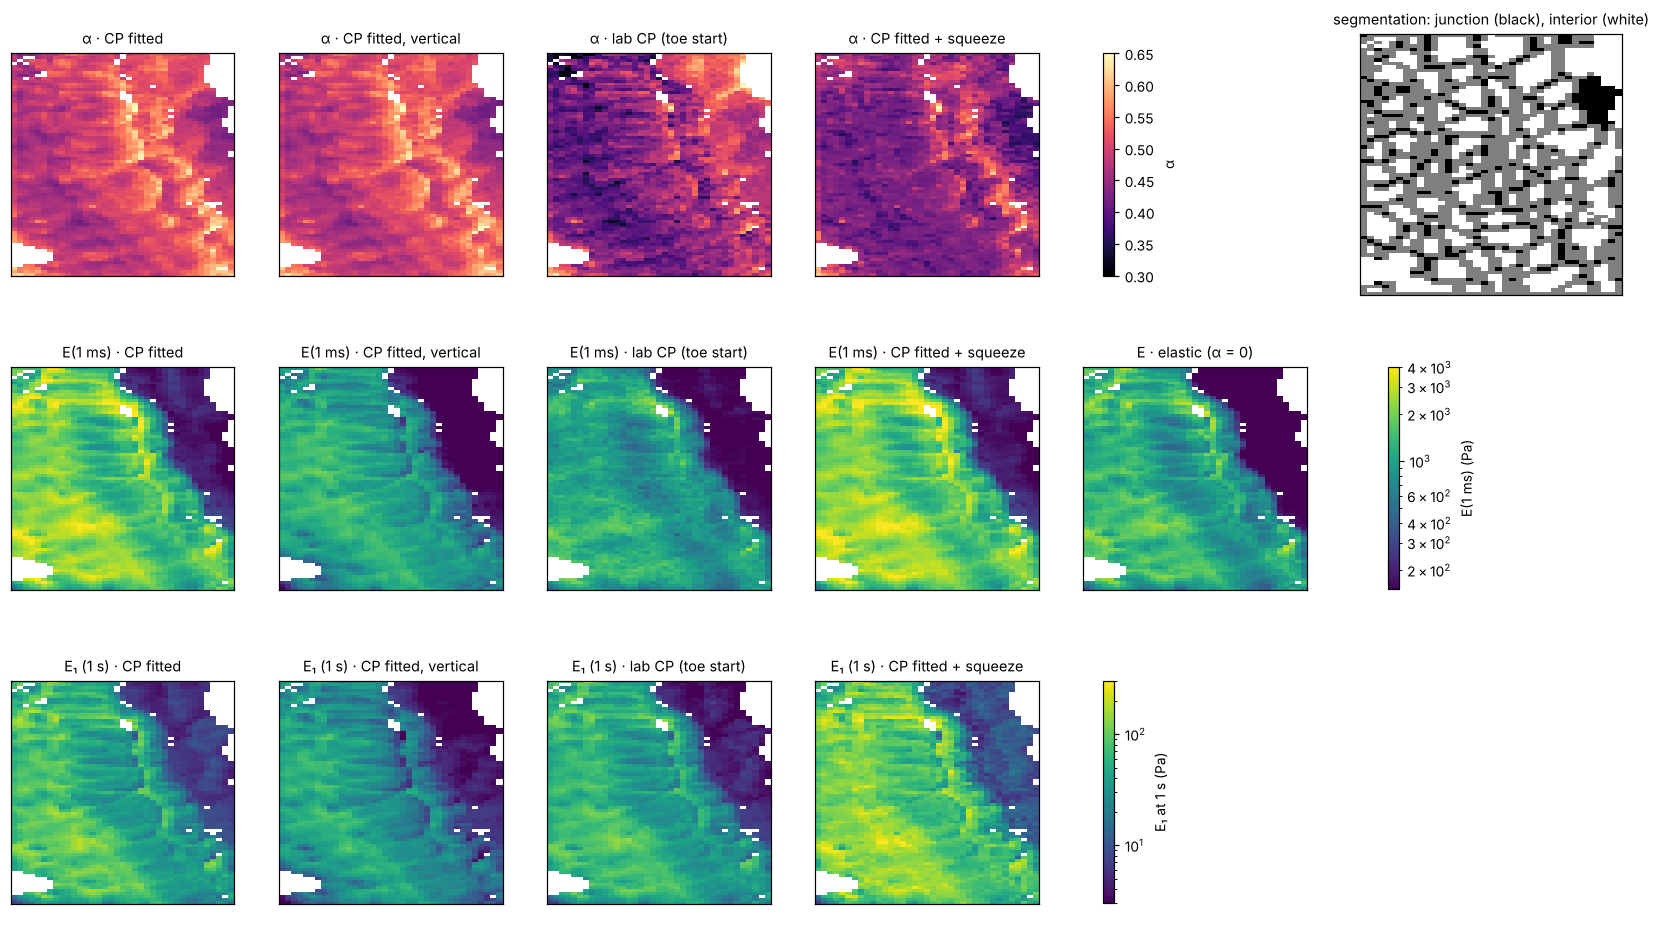
\includegraphics[height=0.86\textheight]{fig/maps_common.png}
\end{frame}

\begin{frame}{Amplitudes (median over the 2623 valid pixels)}
\small
\centering
\begin{tabular}{@{}l r r r r r@{}}
\toprule
variant & $\alpha$ & $E(\SI{1}{\milli\second})$ & $E(\SI{10}{\milli\second})$ & $E_1(\SI{1}{\second})$ & vs.\ main at 1 ms\\
\midrule
\textcolor{cRed}{CP fitted (main)} & 0.501 & 1595 Pa & 487 Pa & 43.8 Pa & --\\
\textcolor{cOrange}{CP fitted, vertical} & 0.500 & 888 Pa & 272 Pa & 25.9 Pa & $\times0.56$\\
\textcolor{cGreen}{lab CP} & 0.442 & 858 Pa & 316 Pa & 40.8 Pa & $\times0.54$\\
\textcolor{cBlue}{squeeze film} & 0.432 & 1754 Pa & 639 Pa & 83.1 Pa & $\times1.10$\\
elastic ($\alpha=0$) & -- & 965 Pa & & & $\times0.60$\\
\bottomrule
\end{tabular}\\[8pt]
\raggedright
\begin{itemize}
\item \textbf{The order of the variants depends on the reference time.} At \SI{1}{\milli\second}, main and squeeze agree (+10\,\%) and the lab CP is half. At \SI{1}{\second}, the squeeze film is $1.9\times$ the main fit: its $\alpha$ is lower by 0.07, worth $e^{6.9\times0.07}=1.6$, on top of the 1.1 at \SI{1}{\milli\second}.
\item \textbf{The vertical fit is $0.56\times$ the main fit}: the median slope is \SI{39}{\degree}, and $\cos^{5/2}\SI{39}{\degree}\approx0.53$.
\item The lab CP and the elastic fit are both $\approx$ half of the main fit, for different reasons (toe counted as indentation vs.\ no relaxation).
\end{itemize}
\end{frame}

\begin{frame}{Patterns: every map normalised to its own median and spread}
\centering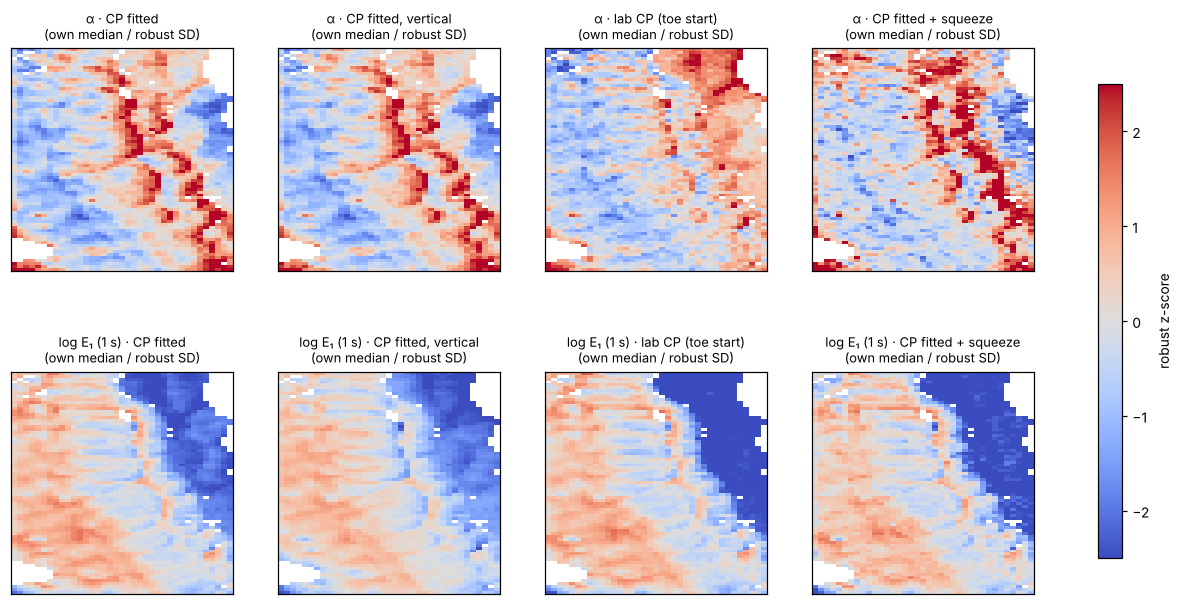
\includegraphics[height=0.68\textheight]{fig/maps_normalised.png}\\
\small
\begin{itemize}
\item \textbf{$\log E_1$}: the same pattern in every variant.
\item \textbf{$\alpha$}: main, vertical and squeeze share the high-$\alpha$ lines. The lab-CP map is dominated by streaks along the scan lines and a different large-scale pattern.
\end{itemize}
\end{frame}

\begin{frame}{Do the variants agree on \emph{where} $E$ and $\alpha$ are high?}
\centering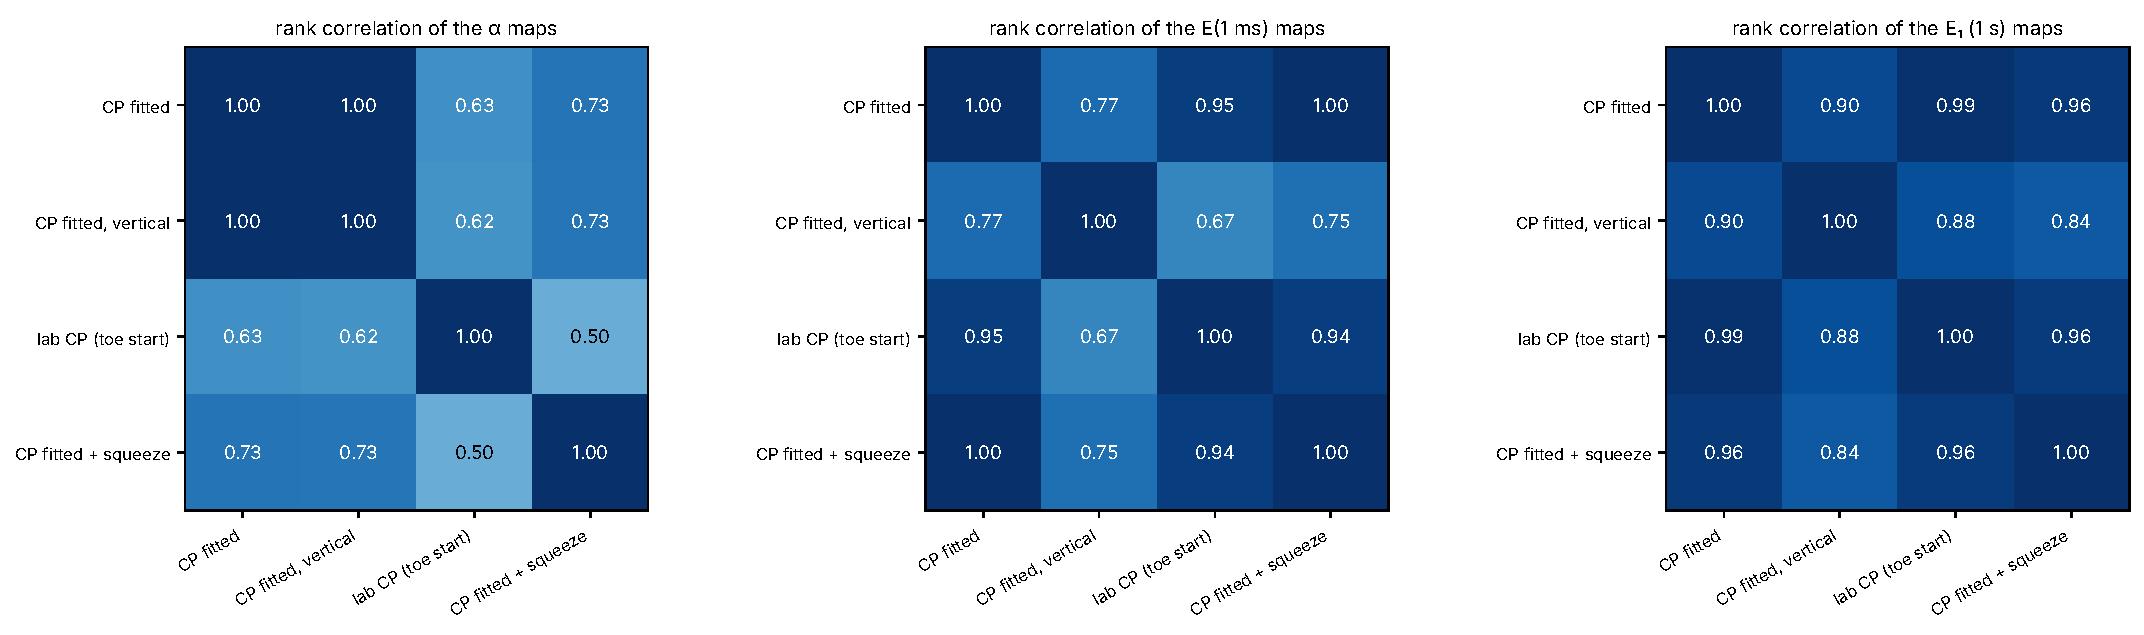
\includegraphics[width=\textwidth]{fig/spearman.pdf}\\[-2pt]
\small
\begin{itemize}
\item \textbf{$E(\SI{1}{\milli\second})$}: the ranking is almost identical for main, squeeze and lab CP ($\rho$ = 0.94--0.996). Only the slope correction changes it ($\rho=0.77$ main vs.\ vertical).
\item \textbf{$\alpha$}: the rankings differ ($\rho$ = 0.50--0.74 between contact-point treatments). Which pixels count as ``more fluid-like'' depends on the method.
\item \textbf{$E_1$ (\SI{1}{\second})}: high agreement ($\rho\ge0.96$ except vertical). $E_1$ is dominated by the large-scale stiffness pattern, which all variants see.
\end{itemize}
\end{frame}

\begin{frame}{Contrast: spread across the map and junction vs.\ cell interior}
\centering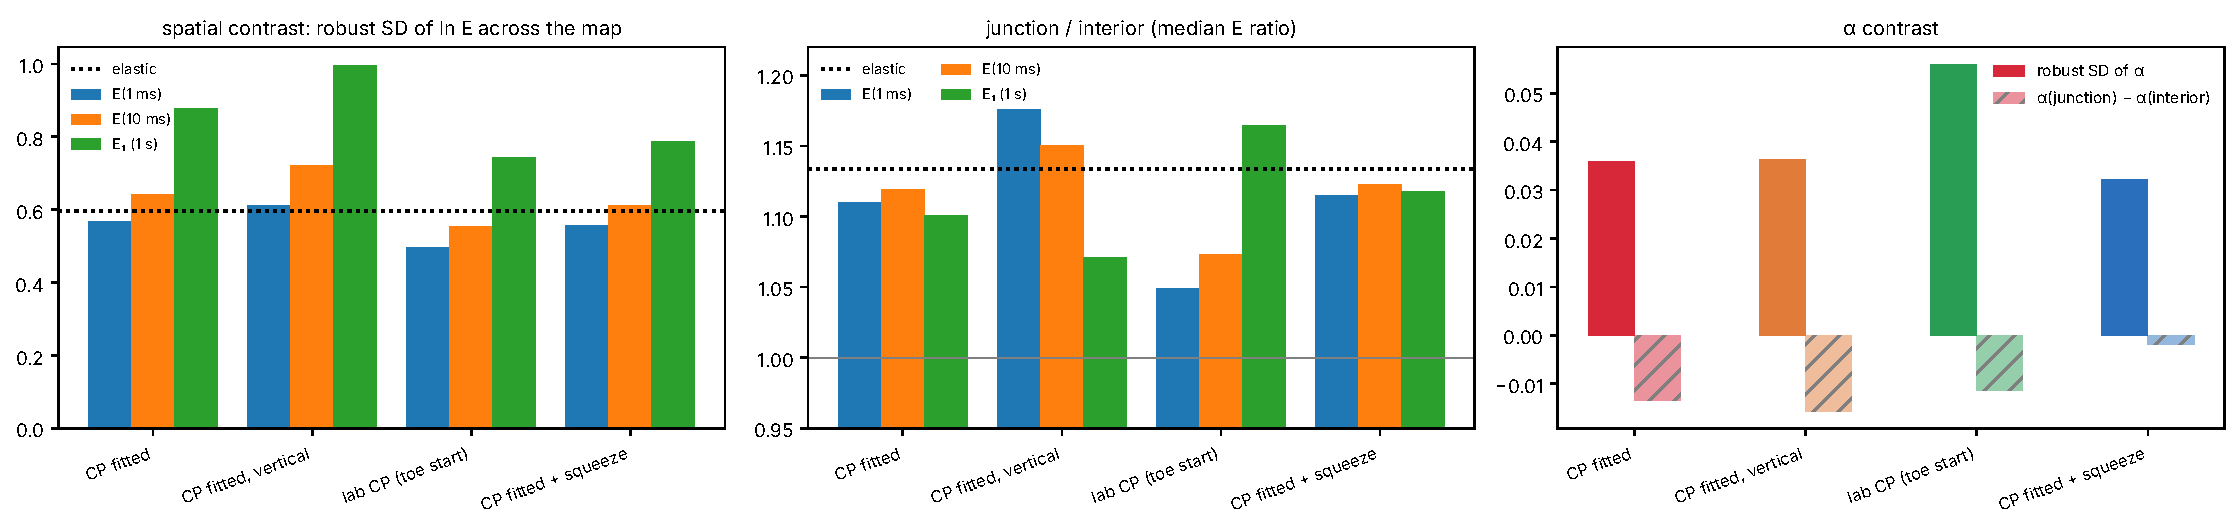
\includegraphics[width=\textwidth]{fig/contrast.pdf}\\
\scriptsize
\begin{tabular}{@{}l c c c | c c c | c c@{}}
\toprule
 & \multicolumn{3}{c|}{robust SD of $\ln E$} & \multicolumn{3}{c|}{$E$ junction / interior} & \multicolumn{2}{c}{$\alpha$}\\
variant & 1 ms & 10 ms & 1 s & 1 ms & 10 ms & 1 s & robust SD & junct.$-$int.\\
\midrule
main & 0.57 & 0.64 & 0.88 & 1.11 & 1.12 & 1.10 & 0.036 & $-0.014$\\
vertical & 0.61 & 0.72 & 1.00 & 1.18 & 1.15 & 1.07 & 0.036 & $-0.016$\\
lab CP & 0.50 & 0.55 & 0.74 & 1.05 & 1.07 & 1.16 & 0.056 & $-0.011$\\
squeeze & 0.56 & 0.61 & 0.79 & 1.11 & 1.12 & 1.12 & 0.032 & $-0.002$\\
elastic & 0.60 & & & 1.13 & & & & \\
\bottomrule
\end{tabular}\\[2pt]
\small Junction and interior are taken from the cell segmentation of this frame (343 junction and 852 interior pixels).
\end{frame}

\begin{frame}{Reading the contrast numbers}
\small
\begin{itemize}
\item \textbf{The contrast of $E$ grows with the reference time} (main: 0.57 $\to$ 0.64 $\to$ 0.88). This is not more information: $\ln E(t)=\ln E(\SI{1}{\milli\second})-\alpha\ln(t/\SI{1}{\milli\second})$, so the variation of $\alpha$ is added with weight 6.9 at \SI{1}{\second}. At \SI{1}{\second}, more than half of the variance of $\ln E$ across the map ($0.88^2$ vs.\ $0.57^2$) is extrapolated $\alpha$.
\item \textbf{The lab CP lowers the $E$ contrast} (0.50 vs.\ 0.57 at 1 ms), and the junction/interior ratio changes from 1.05 at 1 ms to 1.16 at 1 s. Its $\alpha$ spread is the largest (0.056), from the streaks.
\item \textbf{Junctions are $\approx11\,\%$ stiffer than cell interiors} at \SI{1}{\milli\second} in main and squeeze (vertical 18\,\%, lab 5\,\%).
\item \textbf{$\alpha$ at junctions vs.\ interiors}: hardly different in any variant ($\le0.016$). The high-$\alpha$ lines in the $\alpha$ maps are \emph{not} the segmented junctions. They are only weakly related to the surface slope ($r=0.24$), and their origin is open.
\item \textbf{The squeeze film removes most of the $\alpha$ structure at junctions} ($-0.002$). Part of the $\alpha$ contrast in the main fit is toe-related.
\end{itemize}
\end{frame}

% ===========================================================================
\section{$E$ over $\alpha$}

\begin{frame}{$E$ vs.\ $\alpha$ per variant and reference time}
\centering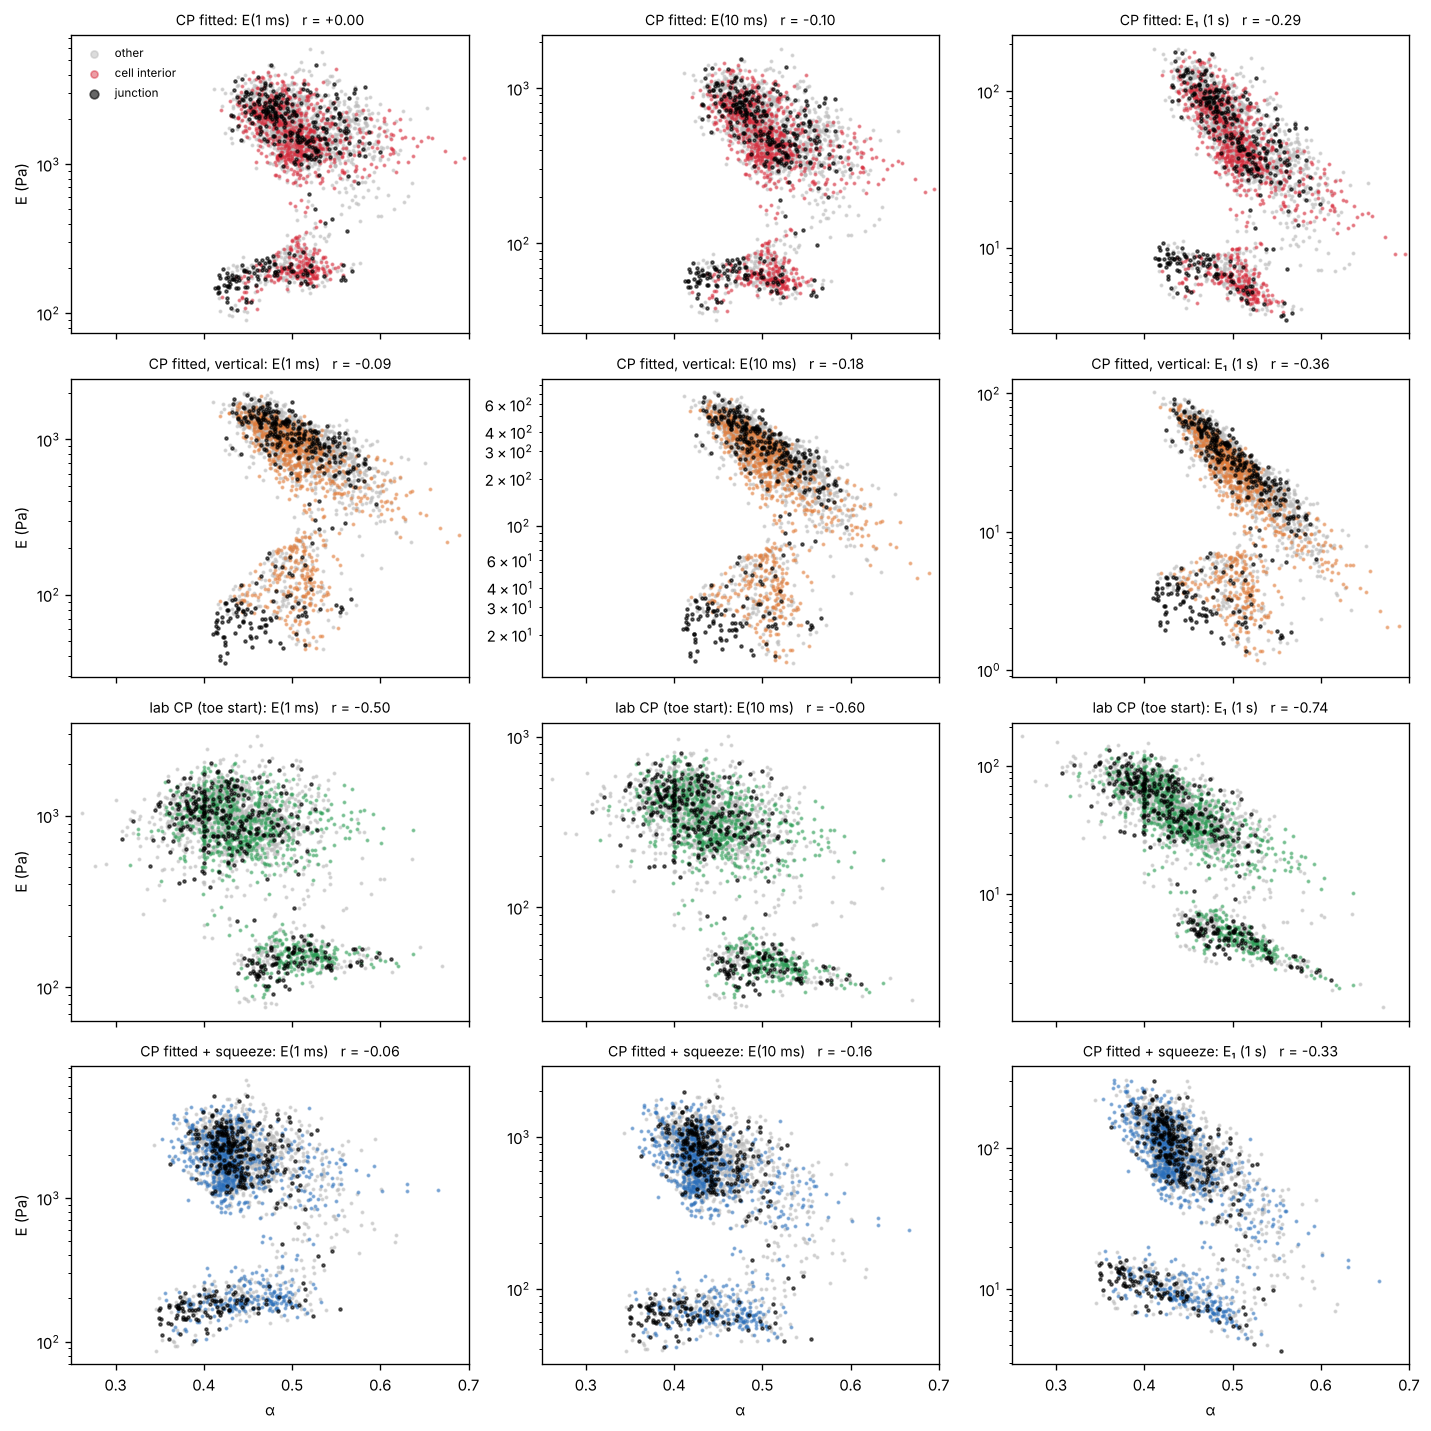
\includegraphics[height=0.86\textheight]{fig/E_vs_alpha.png}
\end{frame}

\begin{frame}{What the $E$--$\alpha$ plots show}
\small
\begin{itemize}
\item \textbf{Two populations}: the embryo surface ($E(\SI{1}{\milli\second})>\SI{500}{\pascal}$, 2125 pixels) and the soft region at the top right (498 pixels). Within each, the trends differ. The whole-map $r$ (e.g.\ 0.00 for main at 1 ms) is an average of opposite trends and is meaningless.
\item \textbf{Within the embryo surface}, $\mathrm{corr}(\log E(t),\alpha)$:
\end{itemize}
\centering
\begin{tabular}{@{}l r r r | r r@{}}
\toprule
variant & 1 ms & 10 ms & 1 s & median $\alpha$ & median $E$(1 ms)\\
\midrule
main & $-0.39$ & $-0.57$ & $-0.77$ & 0.501 & 1814 Pa\\
vertical & $-0.72$ & $-0.81$ & $-0.91$ & 0.500 & 987 Pa\\
lab CP & $-0.09$ & $-0.37$ & $-0.72$ & 0.429 & 960 Pa\\
squeeze & $-0.31$ & $-0.49$ & $-0.72$ & 0.431 & 1968 Pa\\
\bottomrule
\end{tabular}
\raggedright
\begin{itemize}
\item The correlation gets more negative with the reference time in \emph{every} variant. This follows from $\log E(t)=\log E_1-\alpha\log t$ alone: the cloud rotates.
\item \textbf{The slope correction matters}: without it (vertical) the coupling is strongest. On tilted surfaces, the force and indentation errors act on $E$ and $\alpha$ together.
\end{itemize}
\end{frame}

\begin{frame}{Correlation as a function of the reference time}
\begin{columns}[T]
\begin{column}{0.55\textwidth}
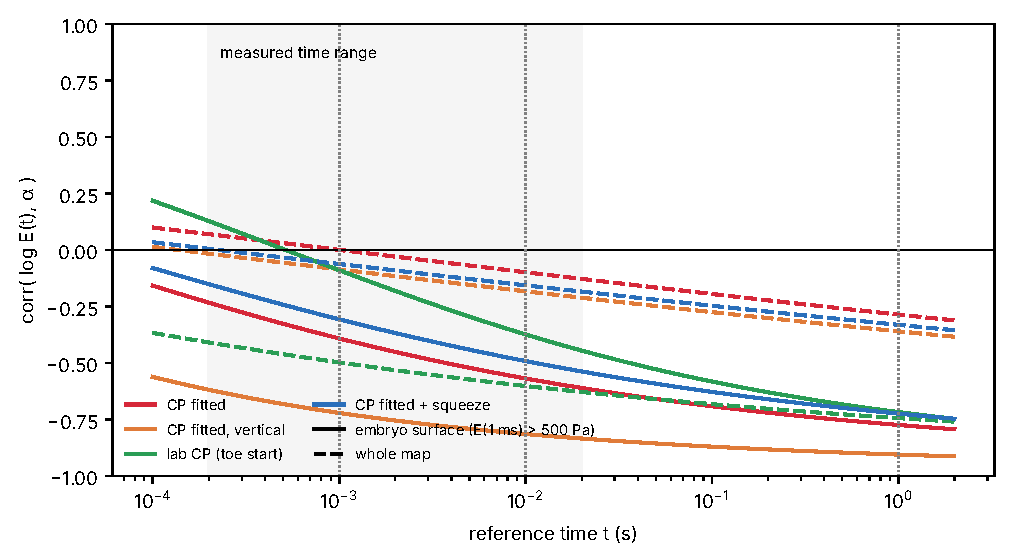
\includegraphics[width=\textwidth]{fig/corr_vs_t.pdf}
\end{column}
\begin{column}{0.43\textwidth}\small
\begin{itemize}
\item \textbf{Whole map (dashed)}: the correlation crosses zero at 0.1--1 ms depending on the variant. This crossing comes from the two populations, not from physics.
\item \textbf{Embryo surface (solid)}: main, vertical and squeeze are negative at every reference time from 0.1 ms to 2 s. The lab CP crosses zero at 0.5 ms.
\item \textbf{Fit noise} alone would give a pivot at $t_c\approx\SI{1.7}{\milli\second}$, but its size is negligible ($\sigma_\alpha\approx0.0004$).
\item So the remaining negative correlation on the embryo surface is systematic or biological. The synthetic test shows that the toe alone produces part of it: $\alpha$ is biased up more for softer curves.
\end{itemize}
\end{column}
\end{columns}
\end{frame}

\begin{frame}{Relaxation curves: interior (colour) and junctions (black)}
\centering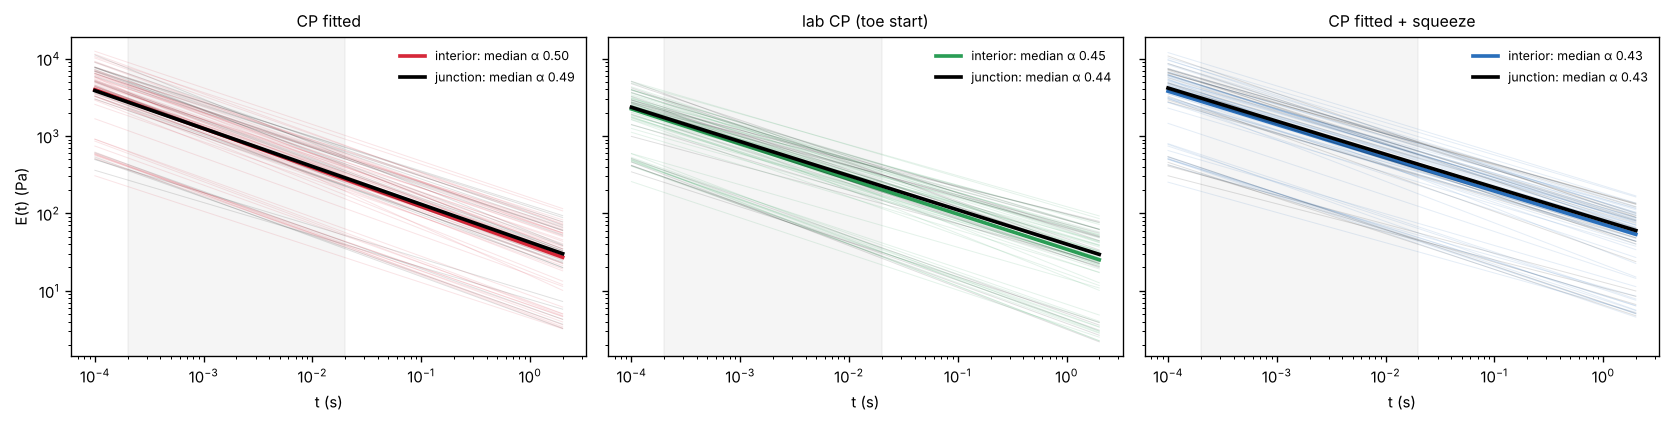
\includegraphics[width=\textwidth]{fig/fans.png}\\
\small
\begin{itemize}
\item Each thin line is $E(t)$ of one pixel; the thick lines are the medians. The grey band is the measured time range.
\item Inside the band the lines are well constrained. Outside it, everything is extrapolation, and the fan widens with distance (the $E_1$ spread at \SI{1}{\second}).
\item Junction and interior medians are nearly parallel ($\alpha$ 0.49 vs.\ 0.50 in the main fit). The junctions are stiffer by an almost constant factor at every time.
\end{itemize}
\end{frame}

% ===========================================================================
\section{Recommendations}

\begin{frame}{What to report}
\footnotesize
\begin{itemize}
\item \textbf{Stiffness}: $E(\SI{1}{\milli\second})$ of the main fit (CP fitted, slope-corrected), with the squeeze-film variant as an uncertainty check.
 \begin{itemize}
 \item The two agree within 10\,\% in amplitude and 0.996 in rank.
 \item Synthetic error $\le4\,\%$.
 \item $E(\SI{1}{\milli\second})$ lies inside the measured time range, where the fit-noise coupling to $\alpha$ is smallest ($t_c\approx\SI{1.7}{\milli\second}$).
 \end{itemize}
\item \textbf{Do not use $E_1$ at \SI{1}{\second}} as a stiffness measure. It is biased by 20--40\,\% and half of its contrast is extrapolated $\alpha$. If a long-time modulus is needed, it requires dwell/relaxation measurements.
\item \textbf{$\alpha$}: use it for comparisons within one data set and one variant. Give the absolute value as ``$\approx0.43$--0.50, likely too high by up to $\approx0.08$ due to the toe force''. Patterns in $\alpha$ that change between the main and squeeze variants (rank correlation 0.74) should not be interpreted.
\item \textbf{$E$--$\alpha$ relationship}:
 \begin{itemize}
 \item analyse each population separately;
 \item state the reference time;
 \item show at least the main and squeeze variants.
 \end{itemize}
 A negative slope is expected even without biology, from the toe bias (softer $\Rightarrow$ $\alpha$ too high) and from the rotation with the reference time.
\item \textbf{Do not use the lab contact point}: it halves $E$, fails the depth check, compresses the $\alpha$ range and adds scan-line streaks.
\end{itemize}
\end{frame}

\begin{frame}{Next steps that would settle the open points}
\small
\begin{enumerate}
\item \textbf{Approach speed series} (e.g.\ 100, 300, \SI{1000}{\micro\metre\per\second}) on one area. A drag force scales with the speed, a soft surface layer does not. This decides between the main and squeeze variants and fixes the absolute $\alpha$.
\item \textbf{Dwell (hold at constant indentation)} for 0.1--1 s: measures $E(t)$ directly up to \SI{1}{\second}, so $E_1$ would no longer be an extrapolation.
\item \textbf{Glass curve} with the same settings: measures the Z--deflection delay (48 µs in the lab pipeline) and the drag baseline without a sample.
\item \textbf{Calibration} of $k$ (thermal tune) and $R$ (SEM or reference sample): these scale every $E$ but leave $\alpha$ and the contrasts unchanged.
\end{enumerate}
\vspace{6pt}
Scripts that made every number and figure in these slides are in \texttt{docs/variants/scripts}.
\end{frame}

\end{document}
